\documentclass{standalone}
\usepackage{tikz}
\usetikzlibrary{patterns, positioning}


\begin{document}
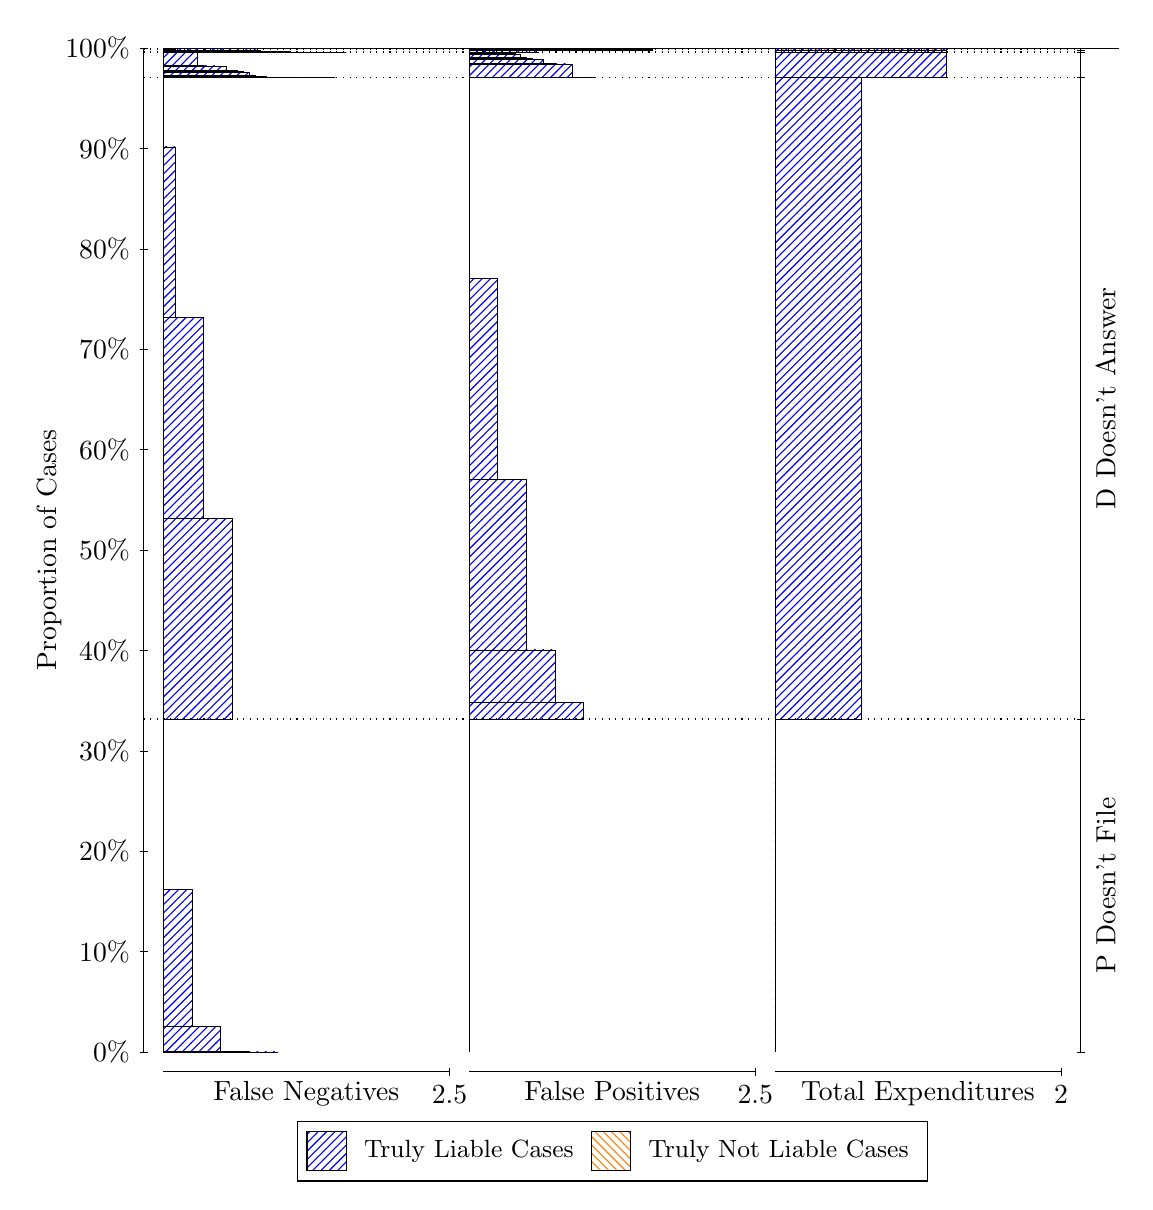
\begin{tikzpicture}
\draw[black, very thin] (1.5,1.75) -- (1.5,14.5);
\node[rotate=90, text=black, anchor=center] at (0.3, 8.125) {Proportion of Cases};
\draw[black, very thin] (1.45,1.75) -- (1.55,1.75);
\node[text=black, anchor=east] at (1.45, 1.75) {0\%};
\draw[black, very thin] (1.45,3.025) -- (1.55,3.025);
\node[text=black, anchor=east] at (1.45, 3.025) {10\%};
\draw[black, very thin] (1.45,4.3) -- (1.55,4.3);
\node[text=black, anchor=east] at (1.45, 4.3) {20\%};
\draw[black, very thin] (1.45,5.575) -- (1.55,5.575);
\node[text=black, anchor=east] at (1.45, 5.575) {30\%};
\draw[black, very thin] (1.45,6.85) -- (1.55,6.85);
\node[text=black, anchor=east] at (1.45, 6.85) {40\%};
\draw[black, very thin] (1.45,8.125) -- (1.55,8.125);
\node[text=black, anchor=east] at (1.45, 8.125) {50\%};
\draw[black, very thin] (1.45,9.4) -- (1.55,9.4);
\node[text=black, anchor=east] at (1.45, 9.4) {60\%};
\draw[black, very thin] (1.45,10.675) -- (1.55,10.675);
\node[text=black, anchor=east] at (1.45, 10.675) {70\%};
\draw[black, very thin] (1.45,11.95) -- (1.55,11.95);
\node[text=black, anchor=east] at (1.45, 11.95) {80\%};
\draw[black, very thin] (1.45,13.225) -- (1.55,13.225);
\node[text=black, anchor=east] at (1.45, 13.225) {90\%};
\draw[black, very thin] (1.45,14.5) -- (1.55,14.5);
\node[text=black, anchor=east] at (1.45, 14.5) {100\%};

\draw[black, very thin] (13.4,1.75) -- (13.4,14.5);
\draw[black, very thin] (13.35,1.75) -- (13.45,1.75);
\node[anchor=west] at (13.35, 1.75) {};
\draw[black, very thin] (13.35,5.9785) -- (13.45,5.9785);
\node[anchor=west] at (13.35, 5.9785) {};
\draw[black, very thin] (13.35,14.123) -- (13.45,14.123);
\node[anchor=west] at (13.35, 14.123) {};
\draw[black, very thin] (13.35,14.449) -- (13.45,14.449);
\node[anchor=west] at (13.35, 14.449) {};
\draw[black, very thin] (13.35,14.476) -- (13.45,14.476);
\node[anchor=west] at (13.35, 14.476) {};
\draw[black, very thin] (13.35,14.498) -- (13.45,14.498);
\node[anchor=west] at (13.35, 14.498) {};
\draw[black, very thin] (13.35,14.5) -- (13.45,14.5);
\node[anchor=west] at (13.35, 14.5) {};

\draw[black, very thin, pattern color=blue, pattern=north east lines] (1.75,1.75) rectangle (3.2033,1.75);
\draw[black, very thin, pattern color=blue, pattern=north east lines] (1.75,1.75) rectangle (2.84,1.7528);
\draw[black, very thin, pattern color=blue, pattern=north east lines] (1.75,1.7528) rectangle (2.4767,2.0766);
\draw[black, very thin, pattern color=blue, pattern=north east lines] (1.75,2.0766) rectangle (2.1133,3.8168);
\draw[black, very thin, pattern color=orange, pattern=north west lines] (1.75,3.8168) rectangle (1.75,3.8168);
\draw[black, very thin, pattern color=blue, pattern=north east lines] (1.75,3.8168) rectangle (1.75,5.9785);
\draw[black, very thin, pattern color=blue, pattern=north east lines] (1.75,5.9785) rectangle (2.622,8.5284);
\draw[black, very thin, pattern color=blue, pattern=north east lines] (1.75,8.5284) rectangle (2.2587,11.075);
\draw[black, very thin, pattern color=blue, pattern=north east lines] (1.75,11.075) rectangle (1.8953,13.245);
\draw[black, very thin, pattern color=orange, pattern=north west lines] (1.75,13.245) rectangle (1.75,13.245);
\draw[black, very thin, pattern color=blue, pattern=north east lines] (1.75,13.245) rectangle (1.75,14.123);
\draw[black, very thin, pattern color=blue, pattern=north east lines] (1.75,14.123) rectangle (3.93,14.123);
\draw[black, very thin, pattern color=blue, pattern=north east lines] (1.75,14.123) rectangle (3.7847,14.123);
\draw[black, very thin, pattern color=blue, pattern=north east lines] (1.75,14.123) rectangle (3.6393,14.123);
\draw[black, very thin, pattern color=blue, pattern=north east lines] (1.75,14.123) rectangle (3.5667,14.123);
\draw[black, very thin, pattern color=blue, pattern=north east lines] (1.75,14.123) rectangle (3.494,14.123);
\draw[black, very thin, pattern color=blue, pattern=north east lines] (1.75,14.123) rectangle (3.4213,14.123);
\draw[black, very thin, pattern color=blue, pattern=north east lines] (1.75,14.123) rectangle (3.3487,14.123);
\draw[black, very thin, pattern color=blue, pattern=north east lines] (1.75,14.123) rectangle (3.276,14.123);
\draw[black, very thin, pattern color=blue, pattern=north east lines] (1.75,14.123) rectangle (3.2033,14.13);
\draw[black, very thin, pattern color=blue, pattern=north east lines] (1.75,14.13) rectangle (3.1307,14.13);
\draw[black, very thin, pattern color=blue, pattern=north east lines] (1.75,14.13) rectangle (3.058,14.143);
\draw[black, very thin, pattern color=blue, pattern=north east lines] (1.75,14.143) rectangle (2.9853,14.143);
\draw[black, very thin, pattern color=blue, pattern=north east lines] (1.75,14.143) rectangle (2.9127,14.156);
\draw[black, very thin, pattern color=blue, pattern=north east lines] (1.75,14.156) rectangle (2.84,14.194);
\draw[black, very thin, pattern color=blue, pattern=north east lines] (1.75,14.194) rectangle (2.7673,14.201);
\draw[black, very thin, pattern color=blue, pattern=north east lines] (1.75,14.201) rectangle (2.6947,14.214);
\draw[black, very thin, pattern color=blue, pattern=north east lines] (1.75,14.214) rectangle (2.622,14.219);
\draw[black, very thin, pattern color=blue, pattern=north east lines] (1.75,14.219) rectangle (2.5493,14.265);
\draw[black, very thin, pattern color=blue, pattern=north east lines] (1.75,14.265) rectangle (2.4767,14.267);
\draw[black, very thin, pattern color=blue, pattern=north east lines] (1.75,14.267) rectangle (2.404,14.273);
\draw[black, very thin, pattern color=blue, pattern=north east lines] (1.75,14.273) rectangle (2.3313,14.273);
\draw[black, very thin, pattern color=blue, pattern=north east lines] (1.75,14.273) rectangle (2.2587,14.276);
\draw[black, very thin, pattern color=blue, pattern=north east lines] (1.75,14.276) rectangle (2.186,14.449);
\draw[black, very thin, pattern color=blue, pattern=north east lines] (1.75,14.449) rectangle (2.0407,14.449);
\draw[black, very thin, pattern color=blue, pattern=north east lines] (1.75,14.449) rectangle (1.8953,14.449);
\draw[black, very thin, pattern color=orange, pattern=north west lines] (1.75,14.449) rectangle (1.75,14.449);
\draw[black, very thin, pattern color=blue, pattern=north east lines] (1.75,14.449) rectangle (4.0753,14.449);
\draw[black, very thin, pattern color=blue, pattern=north east lines] (1.75,14.449) rectangle (3.712,14.449);
\draw[black, very thin, pattern color=blue, pattern=north east lines] (1.75,14.449) rectangle (3.3487,14.454);
\draw[black, very thin, pattern color=blue, pattern=north east lines] (1.75,14.454) rectangle (2.9853,14.475);
\draw[black, very thin, pattern color=blue, pattern=north east lines] (1.75,14.475) rectangle (2.622,14.476);
\draw[black, very thin, pattern color=orange, pattern=north west lines] (1.75,14.476) rectangle (1.75,14.476);
\draw[black, very thin, pattern color=blue, pattern=north east lines] (1.75,14.476) rectangle (2.622,14.476);
\draw[black, very thin, pattern color=blue, pattern=north east lines] (1.75,14.476) rectangle (2.2587,14.477);
\draw[black, very thin, pattern color=blue, pattern=north east lines] (1.75,14.477) rectangle (1.8953,14.482);
\draw[black, very thin, pattern color=orange, pattern=north west lines] (1.75,14.482) rectangle (1.75,14.482);
\draw[black, very thin, pattern color=blue, pattern=north east lines] (1.75,14.482) rectangle (1.75,14.498);
\draw[black, very thin, pattern color=blue, pattern=north east lines] (1.75,14.498) rectangle (5.8193,14.498);
\draw[black, very thin, pattern color=blue, pattern=north east lines] (1.75,14.498) rectangle (5.456,14.498);
\draw[black, very thin, pattern color=blue, pattern=north east lines] (1.75,14.498) rectangle (5.0927,14.498);
\draw[black, very thin, pattern color=blue, pattern=north east lines] (1.75,14.498) rectangle (4.7293,14.498);
\draw[black, very thin, pattern color=blue, pattern=north east lines] (1.75,14.498) rectangle (4.366,14.499);
\draw[black, very thin, pattern color=blue, pattern=north east lines] (1.75,14.499) rectangle (4.0027,14.499);
\draw[black, very thin, pattern color=blue, pattern=north east lines] (1.75,14.499) rectangle (3.712,14.499);
\draw[black, very thin, pattern color=blue, pattern=north east lines] (1.75,14.499) rectangle (3.3487,14.499);
\draw[black, very thin, pattern color=blue, pattern=north east lines] (1.75,14.499) rectangle (2.9853,14.499);
\draw[black, very thin, pattern color=blue, pattern=north east lines] (1.75,14.499) rectangle (2.622,14.5);
\draw[black, very thin, pattern color=blue, pattern=north east lines] (1.75,14.5) rectangle (2.2587,14.5);
\draw[black, very thin, pattern color=blue, pattern=north east lines] (1.75,14.5) rectangle (1.8953,14.5);
\draw[black, very thin, pattern color=orange, pattern=north west lines] (1.75,14.5) rectangle (1.75,14.5);
\draw[black, very thin, pattern color=blue, pattern=north east lines] (1.75,14.5) rectangle (1.75,14.5);
\draw[black, very thin, pattern color=orange, pattern=north west lines] (5.6333,1.75) rectangle (5.6333,1.75);
\draw[black, very thin, pattern color=blue, pattern=north east lines] (5.6333,1.75) rectangle (5.6333,5.9785);
\draw[black, very thin, pattern color=orange, pattern=north west lines] (5.6333,5.9785) rectangle (7.0867,5.9785);
\draw[black, very thin, pattern color=blue, pattern=north east lines] (5.6333,5.9785) rectangle (7.0867,6.1861);
\draw[black, very thin, pattern color=blue, pattern=north east lines] (5.6333,6.1861) rectangle (6.7233,6.8571);
\draw[black, very thin, pattern color=blue, pattern=north east lines] (5.6333,6.8571) rectangle (6.36,9.0266);
\draw[black, very thin, pattern color=blue, pattern=north east lines] (5.6333,9.0266) rectangle (5.9967,11.573);
\draw[black, very thin, pattern color=blue, pattern=north east lines] (5.6333,11.573) rectangle (5.6333,14.123);
\draw[black, very thin, pattern color=orange, pattern=north west lines] (5.6333,14.123) rectangle (7.232,14.123);
\draw[black, very thin, pattern color=blue, pattern=north east lines] (5.6333,14.123) rectangle (7.232,14.123);
\draw[black, very thin, pattern color=orange, pattern=north west lines] (5.6333,14.123) rectangle (7.0867,14.123);
\draw[black, very thin, pattern color=blue, pattern=north east lines] (5.6333,14.123) rectangle (7.0867,14.123);
\draw[black, very thin, pattern color=orange, pattern=north west lines] (5.6333,14.123) rectangle (6.9413,14.123);
\draw[black, very thin, pattern color=blue, pattern=north east lines] (5.6333,14.123) rectangle (6.9413,14.296);
\draw[black, very thin, pattern color=blue, pattern=north east lines] (5.6333,14.296) rectangle (6.8687,14.299);
\draw[black, very thin, pattern color=orange, pattern=north west lines] (5.6333,14.299) rectangle (6.796,14.299);
\draw[black, very thin, pattern color=blue, pattern=north east lines] (5.6333,14.299) rectangle (6.796,14.299);
\draw[black, very thin, pattern color=blue, pattern=north east lines] (5.6333,14.299) rectangle (6.7233,14.306);
\draw[black, very thin, pattern color=orange, pattern=north west lines] (5.6333,14.306) rectangle (6.6507,14.306);
\draw[black, very thin, pattern color=blue, pattern=north east lines] (5.6333,14.306) rectangle (6.6507,14.307);
\draw[black, very thin, pattern color=blue, pattern=north east lines] (5.6333,14.307) rectangle (6.578,14.353);
\draw[black, very thin, pattern color=blue, pattern=north east lines] (5.6333,14.353) rectangle (6.5053,14.358);
\draw[black, very thin, pattern color=blue, pattern=north east lines] (5.6333,14.358) rectangle (6.4327,14.371);
\draw[black, very thin, pattern color=blue, pattern=north east lines] (5.6333,14.371) rectangle (6.36,14.378);
\draw[black, very thin, pattern color=blue, pattern=north east lines] (5.6333,14.378) rectangle (6.2873,14.416);
\draw[black, very thin, pattern color=blue, pattern=north east lines] (5.6333,14.416) rectangle (6.2147,14.429);
\draw[black, very thin, pattern color=blue, pattern=north east lines] (5.6333,14.429) rectangle (6.142,14.429);
\draw[black, very thin, pattern color=blue, pattern=north east lines] (5.6333,14.429) rectangle (6.0693,14.442);
\draw[black, very thin, pattern color=blue, pattern=north east lines] (5.6333,14.442) rectangle (5.9967,14.442);
\draw[black, very thin, pattern color=blue, pattern=north east lines] (5.6333,14.442) rectangle (5.924,14.449);
\draw[black, very thin, pattern color=blue, pattern=north east lines] (5.6333,14.449) rectangle (5.8513,14.449);
\draw[black, very thin, pattern color=blue, pattern=north east lines] (5.6333,14.449) rectangle (5.7787,14.449);
\draw[black, very thin, pattern color=blue, pattern=north east lines] (5.6333,14.449) rectangle (5.706,14.449);
\draw[black, very thin, pattern color=blue, pattern=north east lines] (5.6333,14.449) rectangle (5.6333,14.449);
\draw[black, very thin, pattern color=orange, pattern=north west lines] (5.6333,14.449) rectangle (6.5053,14.449);
\draw[black, very thin, pattern color=blue, pattern=north east lines] (5.6333,14.449) rectangle (6.5053,14.45);
\draw[black, very thin, pattern color=blue, pattern=north east lines] (5.6333,14.45) rectangle (6.142,14.472);
\draw[black, very thin, pattern color=blue, pattern=north east lines] (5.6333,14.472) rectangle (5.7787,14.476);
\draw[black, very thin, pattern color=blue, pattern=north east lines] (5.6333,14.476) rectangle (5.6333,14.476);
\draw[black, very thin, pattern color=orange, pattern=north west lines] (5.6333,14.476) rectangle (7.9587,14.476);
\draw[black, very thin, pattern color=blue, pattern=north east lines] (5.6333,14.476) rectangle (7.9587,14.481);
\draw[black, very thin, pattern color=blue, pattern=north east lines] (5.6333,14.481) rectangle (7.5953,14.492);
\draw[black, very thin, pattern color=blue, pattern=north east lines] (5.6333,14.492) rectangle (7.232,14.498);
\draw[black, very thin, pattern color=blue, pattern=north east lines] (5.6333,14.498) rectangle (6.8687,14.498);
\draw[black, very thin, pattern color=blue, pattern=north east lines] (5.6333,14.498) rectangle (6.5053,14.498);
\draw[black, very thin, pattern color=orange, pattern=north west lines] (5.6333,14.498) rectangle (9.7027,14.498);
\draw[black, very thin, pattern color=blue, pattern=north east lines] (5.6333,14.498) rectangle (9.7027,14.498);
\draw[black, very thin, pattern color=orange, pattern=north west lines] (5.6333,14.498) rectangle (9.3393,14.498);
\draw[black, very thin, pattern color=blue, pattern=north east lines] (5.6333,14.498) rectangle (9.3393,14.498);
\draw[black, very thin, pattern color=orange, pattern=north west lines] (5.6333,14.498) rectangle (8.976,14.498);
\draw[black, very thin, pattern color=blue, pattern=north east lines] (5.6333,14.498) rectangle (8.976,14.498);
\draw[black, very thin, pattern color=orange, pattern=north west lines] (5.6333,14.498) rectangle (8.6127,14.498);
\draw[black, very thin, pattern color=blue, pattern=north east lines] (5.6333,14.498) rectangle (8.6127,14.499);
\draw[black, very thin, pattern color=blue, pattern=north east lines] (5.6333,14.499) rectangle (8.2493,14.499);
\draw[black, very thin, pattern color=blue, pattern=north east lines] (5.6333,14.499) rectangle (7.886,14.499);
\draw[black, very thin, pattern color=blue, pattern=north east lines] (5.6333,14.499) rectangle (7.5227,14.499);
\draw[black, very thin, pattern color=blue, pattern=north east lines] (5.6333,14.499) rectangle (7.1593,14.499);
\draw[black, very thin, pattern color=orange, pattern=north west lines] (5.6333,14.499) rectangle (6.8687,14.499);
\draw[black, very thin, pattern color=blue, pattern=north east lines] (5.6333,14.499) rectangle (6.8687,14.499);
\draw[black, very thin, pattern color=orange, pattern=north west lines] (5.6333,14.499) rectangle (6.5053,14.499);
\draw[black, very thin, pattern color=blue, pattern=north east lines] (5.6333,14.499) rectangle (6.5053,14.5);
\draw[black, very thin, pattern color=blue, pattern=north east lines] (5.6333,14.5) rectangle (6.142,14.5);
\draw[black, very thin, pattern color=blue, pattern=north east lines] (5.6333,14.5) rectangle (5.7787,14.5);
\draw[black, very thin, pattern color=blue, pattern=north east lines] (5.6333,14.5) rectangle (5.6333,14.5);
\draw[black, very thin, pattern color=orange, pattern=north west lines] (9.5167,1.75) rectangle (9.5167,1.75);
\draw[black, very thin, pattern color=blue, pattern=north east lines] (9.5167,1.75) rectangle (9.5167,5.9785);
\draw[black, very thin, pattern color=orange, pattern=north west lines] (9.5167,5.9785) rectangle (10.607,5.9785);
\draw[black, very thin, pattern color=blue, pattern=north east lines] (9.5167,5.9785) rectangle (10.607,14.123);
\draw[black, very thin, pattern color=orange, pattern=north west lines] (9.5167,14.123) rectangle (11.697,14.123);
\draw[black, very thin, pattern color=blue, pattern=north east lines] (9.5167,14.123) rectangle (11.697,14.132);
\draw[black, very thin, pattern color=orange, pattern=north west lines] (9.5167,14.132) rectangle (11.697,14.132);
\draw[black, very thin, pattern color=blue, pattern=north east lines] (9.5167,14.132) rectangle (11.697,14.449);
\draw[black, very thin, pattern color=orange, pattern=north west lines] (9.5167,14.449) rectangle (11.697,14.449);
\draw[black, very thin, pattern color=blue, pattern=north east lines] (9.5167,14.449) rectangle (11.697,14.476);
\draw[black, very thin, pattern color=orange, pattern=north west lines] (9.5167,14.476) rectangle (11.697,14.476);
\draw[black, very thin, pattern color=blue, pattern=north east lines] (9.5167,14.476) rectangle (11.697,14.498);
\draw[black, very thin, pattern color=orange, pattern=north west lines] (9.5167,14.498) rectangle (13.877,14.498);
\draw[black, very thin, pattern color=blue, pattern=north east lines] (9.5167,14.498) rectangle (13.877,14.5);
\draw[black, dotted] (1.5,5.9785) -- (13.4,5.9785);
\draw[black, dotted] (1.5,14.123) -- (13.4,14.123);
\draw[black, dotted] (1.5,14.449) -- (13.4,14.449);
\draw[black, dotted] (1.5,14.476) -- (13.4,14.476);
\draw[black, dotted] (1.5,14.498) -- (13.4,14.498);
\draw[black, very thin] (1.75,1.5) -- (5.3833,1.5);
\node[text=black, anchor=north] at (3.5667, 1.5) {False Negatives};
\draw[black, very thin] (5.3833,1.45) -- (5.3833,1.55);
\node[text=black, anchor=north] at (5.3833, 1.45) {2.5};

\draw[black, very thin] (5.6333,1.5) -- (9.2667,1.5);
\node[text=black, anchor=north] at (7.45, 1.5) {False Positives};
\draw[black, very thin] (9.2667,1.45) -- (9.2667,1.55);
\node[text=black, anchor=north] at (9.2667, 1.45) {2.5};

\draw[black, very thin] (9.5167,1.5) -- (13.15,1.5);
\node[text=black, anchor=north] at (11.333, 1.5) {Total Expenditures};
\draw[black, very thin] (13.15,1.45) -- (13.15,1.55);
\node[text=black, anchor=north] at (13.15, 1.45) {2};

\node[text=black, centered, rotate=90] at (13.72, 3.8643) {P Doesn't File};
\node[text=black, centered, rotate=90] at (13.72, 10.051) {D Doesn't Answer};





\draw (7.449999999999999,1.5) node[draw=none] (baseCoordinate) {};
\begin{scope}[align=center]
        \matrix[scale=0.5, draw=black, below=0.5cm of baseCoordinate, nodes={draw}, column sep=0.1cm]{
            \node[rectangle, draw, minimum width=0.5cm, minimum height=0.5cm, pattern color=blue, pattern=north east lines] {}; &
            \node[draw=none, font=\small, text=black] (B) {Truly Liable Cases}; &
            \node[rectangle, draw, minimum width=0.5cm, minimum height=0.5cm, pattern color=orange, pattern=north west lines] {}; &
            \node[draw=none, font=\small, text=black] (B) {Truly Not Liable Cases}; \\
            };
\end{scope}

\end{tikzpicture}
\end{document}